\documentclass[portrait,a0paper,final,margin=6em]{baposter}
\tracingstats=2
\usepackage[vlined]{algorithm2e}
\usepackage{calc}
\usepackage{graphicx}
\usepackage{amsmath}
\usepackage{amssymb}
\usepackage{relsize}
\usepackage{multirow}
\usepackage{bm}
\usepackage{graphicx}
\usepackage{multicol}
\usepackage{pgfbaselayers}
\pgfdeclarelayer{background}
\pgfdeclarelayer{foreground}
\pgfsetlayers{background,main,foreground}
\usepackage[T1]{fontenc}
\usepackage{times}
\usepackage{helvet}
\usepackage{palatino}
\newcommand{\captionfont}{\footnotesize}
\selectcolormodel{cmyk}
\graphicspath{{images/}}

%%%%%%%%%%%%%%%%%%%%%%%%%%%%%%%%%%%%%%%%%%%%%%%%%%%%%%%%%%%%%%%%%%%%%%%%%%%%%%%%
%%%% Some math symbols used in the text
%%%%%%%%%%%%%%%%%%%%%%%%%%%%%%%%%%%%%%%%%%%%%%%%%%%%%%%%%%%%%%%%%%%%%%%%%%%%%%%%
\newcommand{\Matrix}[1]{\begin{bmatrix} #1 \end{bmatrix}}
\newcommand{\Vector}[1]{\Matrix{#1}}
\newcommand*{\SET}[1]  {\ensuremath{\mathcal{#1}}}
\newcommand*{\MAT}[1]  {\ensuremath{\mathbf{#1}}}
\newcommand*{\VEC}[1]  {\ensuremath{\bm{#1}}}
\newcommand*{\CONST}[1]{\ensuremath{\mathit{#1}}}
\newcommand*{\norm}[1]{\mathopen\| #1 \mathclose\|}% use instead of $\|x\|$
\newcommand*{\abs}[1]{\mathopen| #1 \mathclose|}% use instead of $\|x\|$
\newcommand*{\absLR}[1]{\left| #1 \right|}% use instead of $\|x\|$
\def\norm#1{\mathopen\| #1 \mathclose\|}% use instead of $\|x\|$
\newcommand{\normLR}[1]{\left\| #1 \right\|}% use instead of $\|x\|$

\setlength{\columnsep}{0.7em}
\setlength{\columnseprule}{0mm}

\newcommand{\compresslist}{%
\setlength{\itemsep}{1pt}%
\setlength{\parskip}{0pt}%
\setlength{\parsep}{0pt}%
}
\begin{document}

\typeout{Poster Starts}
%\background{
%  \begin{tikzpicture}[remember picture,overlay]%
%    \draw (current page.north west)+(-2em,-0em) node[anchor=north west] {\hspace{-2em}\includegraphics[height=1.1\textheight]{silhouettes_background}};
%  \end{tikzpicture}%
%}

\definecolor{silver}{cmyk}{0,0,0,0.3}
\definecolor{yellow}{cmyk}{0,0,0.9,0.0}
\definecolor{reddishyellow}{cmyk}{0,0.22,1.0,0.0}
\definecolor{black}{cmyk}{0,0,0.0,1.0}
\definecolor{darkYellow}{cmyk}{0,0,1.0,0.5}
\definecolor{darkSilver}{cmyk}{0,0,0,0.1}
\definecolor{lightyellow}{cmyk}{0,0,0.3,0.0}
\definecolor{lighteryellow}{cmyk}{0,0,0.1,0.0}
\definecolor{lighteryellow}{cmyk}{0,0,0.1,0.0}
\definecolor{lightestyellow}{cmyk}{0,0,0.05,0.0}

\newlength{\leftimgwidth}

\begin{poster}{
  grid=no,
  colspacing=1em,
  bgColorOne=lighteryellow,
  bgColorTwo=lightestyellow,
  borderColor=reddishyellow,
  headerColorOne=yellow,
  headerColorTwo=reddishyellow,
  headerFontColor=black,
  boxColorOne=lightyellow,
  boxColorTwo=lighteryellow,
  textborder=roundedleft,
  %eyecatcher=no,
  headerborder=open,
  headerheight=0.07\textheight,
  headershape=roundedright,
  headershade=plain,
  headerfont=\Large\textsf, %Sans Serif
  boxshade=plain,
  %background=shade-tb,
  background=plain,
  linewidth=2pt
  }
  {
      \includegraphics[width=0.1\linewidth]{UOI-logo}   
  }
  % Title
  {\sf %Sans Serif
  \bf% Serif
  \LARGE\bf{{InFeRno - an Intelligent Framework \\ for Recognizing Pornographic Web Pages}}}
  {\sf %Sans Serif
  	\vspace{-0.01em}\large{Sotiris Karavarsamis, Nikos Ntarmos and Konstantinos Blekas  \\
     [-0.3em]\normalsize University of Ioannina, Greece}\\
     [-0.3em]\small \{cs061205, ntarmos, kblekas\}@cs.uoi.gr   }
  {
      \includegraphics[width=0.11\linewidth,height=3em]{ecml2011}   
  }

  \tikzstyle{light shaded}=[top color=baposterBGtwo!30!white,bottom color=baposterBGone!30!white,shading=axis,shading angle=30]

    \newcommand{\colouredcircle}[1]{%
      \tikz{\useasboundingbox (-0.2em,-0.32em) rectangle(0.2em,0.32em); \draw[draw=black,fill=baposterBGone!80!black!#1!white,line width=0.03em] (0,0) circle(0.18em);}}

  \headerbox{Problem preliminaries}{name=problem,column=0}{
    \large
	\vspace{0.35 cm}
	\begin{itemize}
		\item We propose \textit{InFeRno}, an intelligent web
		pornography elimination system, classifying web pages based
		solely on their visual content
		
		\item Despite the plethora of useful information scattered on
		the Web, the Internet has become a hostile place for unprotected
		people like children
		
		\item The main characteristics of our system are
		
		\begin{itemize}
			\item A minimal but powerful vector space
			\item An extra 'bikini' class that is observed to improve SVM performance
			\item A highly accurate and fast classification system
			\item A full-fledged ICAP-based (Internet Content Adaptation Protocol) implementation of the pornography elimination system
		\end{itemize}
	\end{itemize}
	\vspace{1 cm}
  }

\headerbox{InFeRno architecture}{name=arch,column=1,span=2,row=0}{
	\large
	\begin{center}
		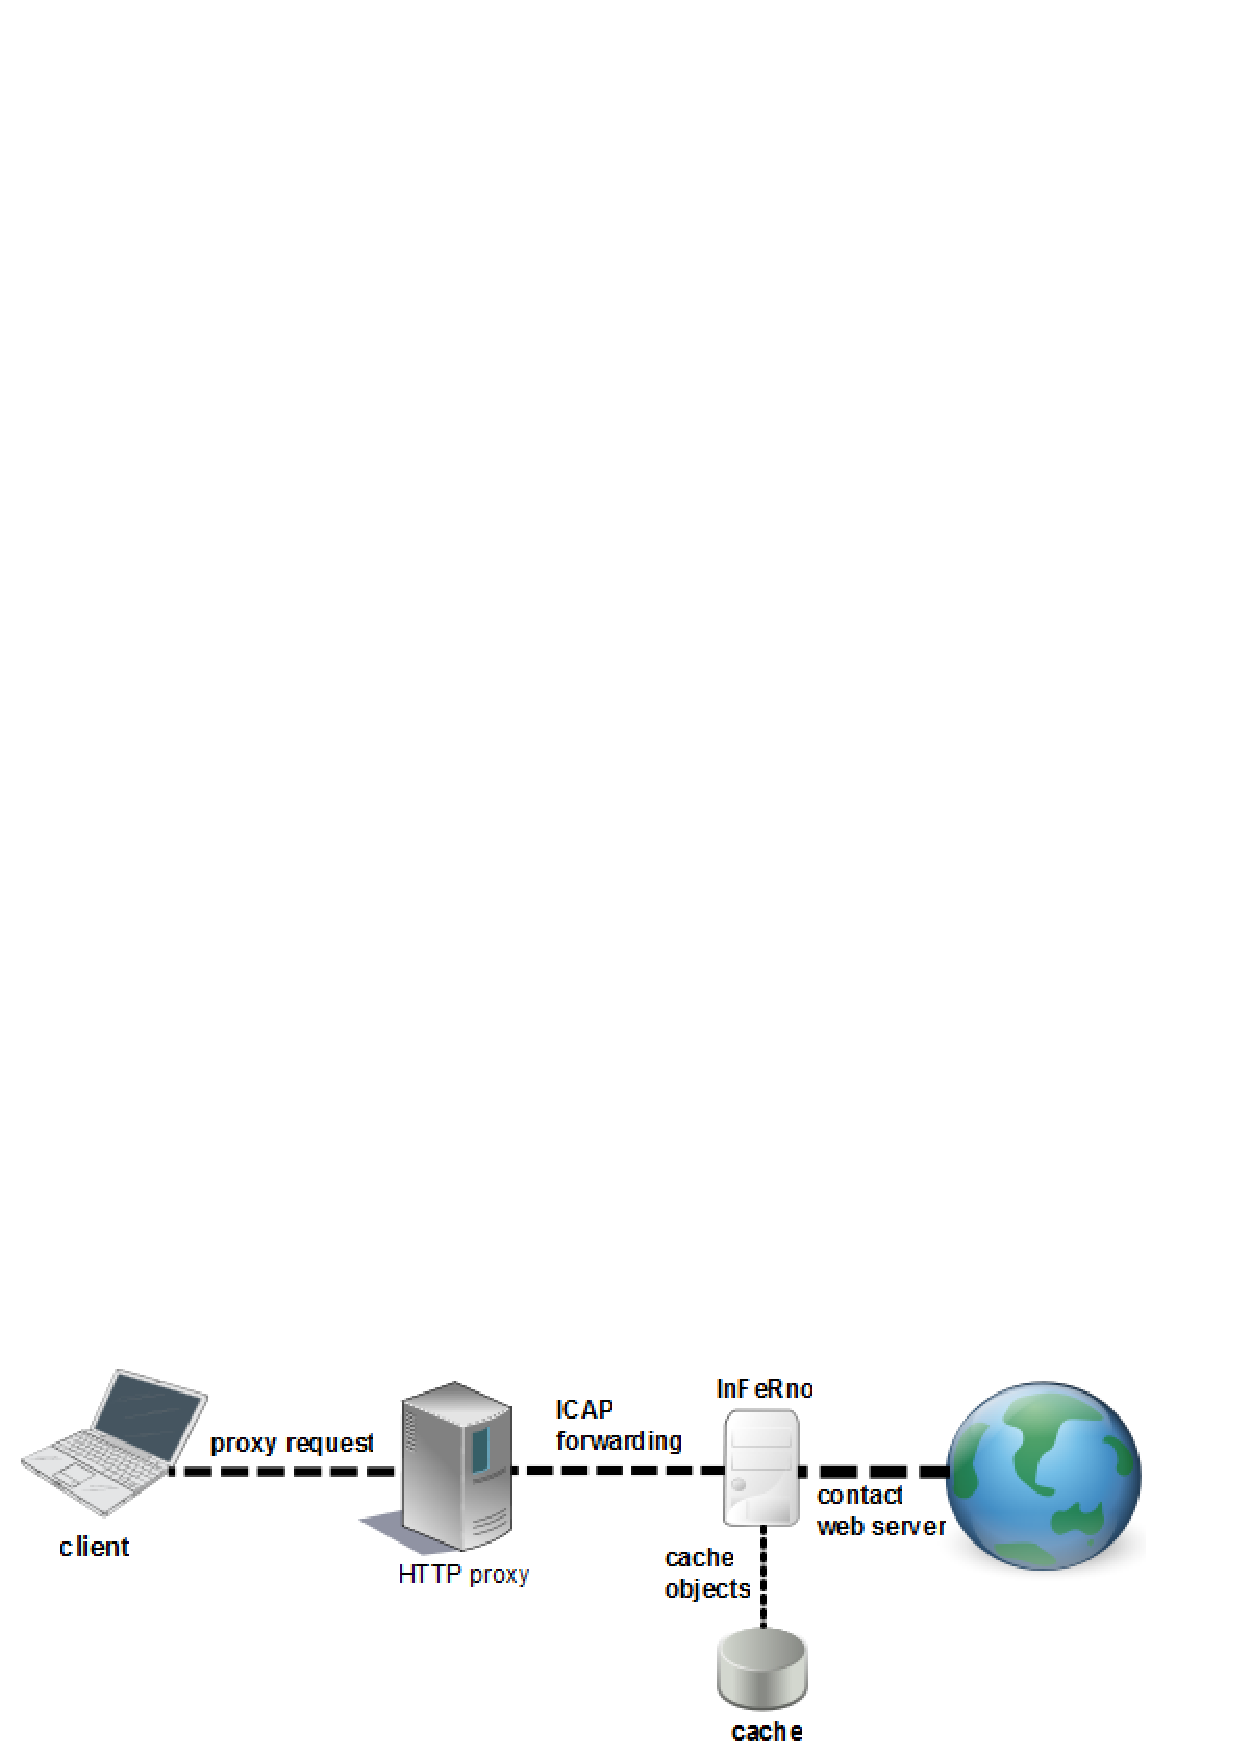
\includegraphics[scale=0.65]{network_diagram.png}
	\end{center}

	\begin{itemize}
		\item Standalone implementation of the InFeRno core as an ICAP module (integrates well with most HTTP proxy servers)
		\item Decoupled image classification and web page pre-processing (network I/O, web content fetching and web page fusion)
		\item A fast ISAM-based cache is implemented for fast cache I/O (classification lookups, updates, etc.)
        \item The administrator can tweak classification and/or network parameters, thus allowing for a flexible setting
	\end{itemize}
	\begin{center}
		\begin{tabular}[c]{cc}
		\ \ \includegraphics[width=.40\columnwidth]{inferno_tp}  \ \ &
		\ \ \includegraphics[width=.40\columnwidth]{ic_tp} \ \ \\
			InFeRno process/thread pool & classifier thread pool\\
		\end{tabular}
	\end{center}
	\vspace{0.3 em}
   }

  \headerbox{References}{name=refs,column=0,span=3,row=2,above=bottom}{
	\begin{enumerate}
		\item POESIA filter project, "Poesia project" http://www.poesia-filter.org/.
		\item W. Hu, O. Wu, Z. Chen, Z. Fu, and S. Maybank, "Recognition
		of pornographic web pages by classifying texts and images",
		\textit{IEEE Trans. on Pattern Analysis and Machine Intelligence}, pp. 1019-1034, 2007.
		\item V. Vezhnevets, V. Sazonov, and A. Andreva, "A survey on
		pixel-based skin color detection techniques," in
		\textit{Graphicon}, pp. 85-92, 2003.
	\end{enumerate}
  }
  \headerbox{Experimental results}{name=expres,column=1,span=2,row=1,below=arch,above=refs}{
	\large
	%\vspace{0.5 cm}
	\begin{itemize}
		\item Training dataset: manually collected 680 bikini images,
		660 porn images and 4260 benign images from the Web
		\item Comparison with the \textit{POESIA filter package} [1]
		\item Results:
			\begin{center}
				\begin{tabular}[c]{c}
					\includegraphics[scale=1.7]{scatter-p-t-all-bars.pdf}
				\end{tabular}
			\end{center}
			
			\begin{itemize}
				\item \textbf{$4\times$ speedup} improvement
				\item Accuracy: 98\% for porn, 97\% for bikini, 98.8\%
				for benign class (comparable to POESIA filter)
			\end{itemize}
	\end{itemize}
    %\vspace{9.5 mm}
  }%

  \headerbox{Classification system}{name=imclass,column=0,span=1,row=1,below=problem,above=refs}{
	\large
	%\vspace{1 cm}
	{
	\normalsize
	\begin{center}
		\begin{tabular}[c]{ccc}
		\ \ 
\includegraphics[width=.15\columnwidth]{orig.pdf}  \ \ &
		\ \ 
\includegraphics[width=.15\columnwidth]{skin.pdf} \ \ &
		\ \ 
\includegraphics[width=.15\columnwidth]{grid.pdf} \ \ \\
			original & skin & contour \\
			image & detection & extraction\\
		\end{tabular}
		%\caption{The image processing steps.} %%
		%\label{RealResults_A}
	\end{center}
	}
	
		Three stages
			\begin{itemize}
				\item Skin detection [3] (Rule-based)
				\item Contour extraction [2] (region splitting scheme)
				\item Feature extraction and Classification
					\begin{itemize}
						\item Extracted 15 features: RGB color statistics, skin-to-nonskin ratio, contour orientation, Hu moments
						\item SVM classifier with RBF kernel
					\end{itemize}
			\end{itemize}
	}
\end{poster}
\end{document}
